\chapter{Rule Set Language}\indexmain{rule set language}
\label{chaprulelang}

The \indexed{rule set} language forms the core of \GrG.
Rule files refer to zero
\footnote{Omitting a graph meta model means that \GrG\ uses a \indexed{default graph model}.
The default model consists of the base type \texttt{Node} for vertices and the base type \texttt{Edge} for edges.}
or more \indexed{graph model}s and specify a set of rewrite rules.
The rule language covers the pattern specification and the rewrite specification in the form of the \texttt{replace} or the \texttt{modify} block.
Attributes of graph elements can be re-evaluated during an application of a rule.
The following rewrite rule mentioned in Geiß et al.~\cite{GBGHS:06} gives a rough picture of the language:
%\begin{figure}[tb]
\begin{example}\label{ex:rule:SomeRule}
\begin{grgen}
using SomeModel;

rule SomeRule {
  n1:NodeTypeA;
  n2:NodeTypeA;
  hom(n1, n2);
  n1 --> n2; /*@\label{ex:somerule:graphlet}@*/
  n3:NodeTypeB;
  negative {
    n3 -e1:EdgeTypeA-> n1;
    if {n3.a1 == 42*n2.a1;}
  }
  negative { /*@\label{ex:somerule:secondnac:begin}@*/
    n4:Node\(NodeTypeB);
    n3 -e1:EdgeTypeB-> n4;
    if {typeof(e1) >= EdgeTypeA;}
  } /*@\label{ex:somerule:secondnac:end}@*/
  replace {
    n5:NodeTypeC<n1>;
    n3 -e1:EdgeTypeB-> n5;
    eval {n5.a3 = n3.a1*n1.a2;}
  }
}
\end{grgen}
\end{example}
%\end{figure}
In this chapter we explain the basics of Example~\ref{ex:rule:SomeRule} (\texttt{SomeRule}),
the more advanced constructs are illustrated in chapter \ref{chapadvanced}.
The nested \texttt{negative}s which specify a pattern which must not be available in the host graph are described in Chapter~\ref{cha:nested}


%%%%%%%%%%%%%%%%%%%%%%%%%%%%%%%%%%%%%%%%%%%%%%%%%%%%%%%%%%%%%%%%%%%%%%%%%%%%%%%%%%%%%%%%%%%%%%%%
\section{Building Blocks}
\label{rulebb}

The \GrG\ rule set language is \indexed{case sensitive}. The language makes use of several identifier specializations in order to denominate all the \GrG\ entities.\\
\\
\emph{Ident}, \emph{IdentDecl}\\ \indexmain{identifier}\nopagebreak
A non-empty character sequence of arbitrary length consisting of letters, digits, or underscores. The first character must not be a digit.
\emph{Ident} may be an identifier defined in a graph model (see Section~\ref{modelbb}).
\emph{Ident} and \emph{IdentDecl} differ in their role: While \emph{IdentDecl} is a \emph{defining} occurrence of an identifier, \emph{Ident} is a \emph{using} occurrence.
An \emph{IdentDecl} non-terminal can be annotated\indexmain{annotation}. See Section~\ref{annotations} for annotations of declarations.
\begin{note}
  As in the \GrG\ model language (see note~\ref{note:modeldecl}) every declaration is also a definition. Using an identifier before defining it is allowed. Every used identifier has to be defined exactly once.
\end{note}
\mbox{ }\\
\emph{ModelIdent}, \emph{TypeIdent}, \emph{NodeType}, \emph{EdgeType}\\
These are (semantic) specializations of \emph{Ident}.
\emph{TypeIdent} matches every type identifier, i.e.\ a node type, an edge type, an enumeration type or a primitive type.
All the type identifiers are actually type \emph{expressions}\indexmain{type expression}.
See Section~\ref{typeexpressions} for the use of type expressions.\\

%-----------------------------------------------------------------------------------------------
\subsection{Graphlets}
\label{sct:graphlets}
\begin{rail}
  Graphlet: (GraphletNode (() | Continuation) | Continuation) ';' ;
  Continuation: GraphletEdge (() | (GraphletNode (() | Continuation))) ;
\end{rail}\ixnterm{Graphlet}\ixnterm{Continuation}
A \indexed{graphlet} specifies a connected subgraph.
\GrG\ provides graphlets as a descriptive notation to define both, patterns\indexmain{pattern graph} to search for as well as the subgraphs that replace or modify matched \indexed{spot}s in a host graph\indexmain{replacement graph}.
Any graph can be specified piecewise by a set of graphlets.
In Example~\ref{ex:rule:SomeRule}, line~\ref{ex:somerule:graphlet}, the statement \texttt{n1 --> n2} is the node identifier \texttt{n1} followed by the \indexedsee{continuation}{graphlet} graphlet \texttt{--> n2}.

All the graph elements of a graphlet have \newterm{name}s.
The name is either user-assigned or a unique internal, non-accessible name.
In the second case the graph element is called \newterm{anonymous}.
For illustration purposes we use a \indexed{\texttt{\$<number>}} notation to denote anonymous graph elements in this document.
For example the graphlet \texttt{n1 --> n2} contains an anonymous edge; thus can be understood as \texttt{n1 -\$1:Edge-> n2}.
Names must not be \indexed{redefine}d; once defined, a name is \emph{bound} to a graph element.
We use the term ``\indexed{binding of names}'' because a name not only denotes a graph element of a graphlet but also denotes the mapping of the abstract graph element of a graphlet to a concrete graph element of a host graph.
So graph elements of different names are pair wise distinct except for homomorphically matched\indexmain{homomorphic matching} graph elements (see Section~\ref{patternpart}).
For instance \texttt{v:NodeType1 -e:EdgeType-> w:NodeType2} selects some node of type \texttt{Node\-Type1} that is connected to a node of type \texttt{NodeType2} by an edge of type \texttt{EdgeType} and binds the names \texttt{v}, \texttt{w}, and \texttt{e}.
If \texttt{v} and \texttt{w} are not explicitly marked as homomorphic, the graph elements they bind to are distinct.
Binding of names allows for splitting a single graphlet into multiple graphlets as well as defining cyclic structures.
\begin{example}
The following graphlet (\texttt{n1}, \texttt{n2}, and \texttt{n3} are defined somewhere else)
\begin{grgen}
n1 --> n2 --> n3 <-- n1;
\end{grgen}
is equivalent to
\begin{grgen}
n2 --> n3;
n1 --> n2;
n3 <-- n1;
\end{grgen}
and \texttt{n1 --> n3} is equivalent to \texttt{n3 <-- n1}, of course.
\end{example}
The visibility of names is determined by \indexed{scope}s.
Scopes can be nested.
Names of surrounding scopes are visible in inner scopes.
Usually a scope is defined by \texttt{\{} and \texttt{\}}. %In contrast to pure syntactic scoping, the replace/modify part is a direct inner scope of the pattern part.
In Example~\ref{ex:rule:SomeRule}, lines~\ref{ex:somerule:secondnac:begin}~to~\ref{ex:somerule:secondnac:end}, the negative condition uses \texttt{n3} from the surrounding scope and defines \texttt{n4} and \texttt{e1}.
We may safely reuse the variable name \texttt{e1} in the replace part.

\begin{rail}
GraphletNode: (Ident |
    '.' |
    (() | IdentDecl) ':' ( NodeType | AdvancedNodeTypeConstructs));
\end{rail}\ixnterm{GraphletNode}
Specifies a node\indexmain{node (graphlet)} of type \emph{NodeType}; the alternative advanced node constructs are explained in chapter \ref{chapadvanced}.
The \texttt{.}\ is an anonymous node of the base type \texttt{Node}; remember that every node type has \texttt{Node} as super type.

\begin{center}
  \begin{tabularx}{\linewidth}{lX}
    \textbf{Graphlet} & \textbf{Meaning}\\ \hline
    \texttt{x:NodeType;} & The name \texttt{x} is bound to a node of type \texttt{NodeType} or one of its subtypes. \\
    \texttt{ :NodeType;} & \texttt{\$1:NodeType} \\
    \texttt{.;} & \texttt{\$1:Node} \\
    \texttt{x;} & The node to which \texttt{x} is bound to.
  \end{tabularx}
\end{center}

\begin{rail}
  GraphletEdge: '-' EdgeRefinement '->'  | '<-' EdgeRefinement '-'  | '<-' EdgeRefinement '->' | '?-' EdgeRefinement '-?' | Redirect;
  EdgeRefinement: () | Ident | (() | IdentDecl) ':' ( EdgeType | AdvancedEdgeTypeConstructs);
\end{rail}\ixnterm{GraphletEdge}\ixnterm{EdgeRefinement}
A \emph{GraphletEdge} specifies an edge\indexmain{edge (graphlet)}.
Anonymous edges are specified by an empty \emph{EdgeRefinement} clause, i.\,e.\ \texttt{-->}, \texttt{<--}, \texttt{<-->}, \texttt{--}, \texttt{?--?} or \texttt{-:T->}, \texttt{<-:T-}, \dots\ for an edge type \texttt{T}, respectively.
A non-empty \emph{EdgeRefinement} clause allows for detailed edge type specification.
The alternative advanced edge constructs as well as the \emph{Redirect} clause are explained in chapter \ref{chapadvanced}.

The different kind of arrow tips distinguish between \indexed{directed}, \indexed{undirected}, and \indexed{arbitrary} edges (see also Section~\ref{sct:basetypes}).
The arrows \texttt{-->} and \texttt{<--} are used for directed edges with a defined source and target.
The arrow \texttt{--} is used for undirected edges.
The pattern part allows for further arrow tips, namely \texttt{?--?}\ for arbitrary edges and \texttt{<-->} for directed edges with undefined direction.
Note that \texttt{<-->} is \emph{not} equivalent to the \texttt{--> ; <-- ;} statements.
In order to produce a match for the arrow \texttt{<-->}, it is sufficient that one of the statements \texttt{-->}, \texttt{<--} matches.
If an edge type is specified (through the \emph{EdgeRefinement} clause), this type has to correspond to the arrow tips, of course.
\begin{center}
	\begin{tabularx}{\linewidth}{lX}
		\textbf{Graphlet} & \textbf{Meaning}\\ \hline
		\texttt{ -e:EdgeType-> ;} & The name \texttt{e} is bound to an edge of type \texttt{EdgeType} or one of its subtypes. \\
		\texttt{ -:EdgeType-> ;} & \texttt{-\$1:EdgeType-> ;} \\
		\texttt{ --> ;} & \texttt{-\$1:Edge-> ;} \\
		\texttt{ <--> ;} & \texttt{-\$1:Edge-> ;} or  \texttt{<-\$1:Edge- ;}\\
		\texttt{ -- ;} & \texttt{-\$1:UEdge-> ;} \\
		\texttt{ ?--?\ ;} & \texttt{-\$1:AEdge-> ;} \\
		\texttt{ -e-> ;} & The edge, \texttt{e} is bound to.
	\end{tabularx}
\end{center}
As the above table shows, edges can be defined and used separately, i.e.\ without their incident nodes.
Accidentally ``\indexed{redirecting}'' an edge is prevented by compiler checks (you must explicitely use the \emph{Redirect} clause to achieve this):
The graphlets
\begin{grgenlet}
-e:Edge-> .;
x:Node -e-> y:Node;
\end{grgenlet}
are illegal, because the edge \texttt{e} would have two destinations: an anonymous node and \texttt{y}.
However, the graphlets
\begin{grgenlet}
-e-> ;
x:Node -e:Edge-> y:Node;
\end{grgenlet}
are allowed, but the first graphlet \texttt{-e->} is superfluous. In particular this graphlet does not identify or create any ``copies'', neither if the graphlet occurs in the pattern part nor if it occurs in the replace part.
\begin{example}
Some attempts to specify a loop edge:\\
\mbox{ }\\
\begin{tabular}[c]{ll}
 \textbf{Graphlet} & \textbf{Meaning} \\ \hline
 \texttt{x:Node -e:Edge-> x;} & The edge \texttt{e} is a loop.\\
 \texttt{x:Node -e:Edge-> ; -e-> x;} & The edge \texttt{e} is a loop.\\
 \texttt{-e:Edge-> x:Node;} & The edge \texttt{e} may or may not be a loop.\\
 \texttt{.\ -e:Edge-> .;} & The edge \texttt{e} is certainly not a loop.\\
\end{tabular}
\end{example}

\begin{figure}[htbp]
\begin{example}
\label{ex:somegraphlets}
Some graphlets:

\begin{center}
\begin{tabular}[c]{cl}
  & \\
  \begin{tabular}[c]{c}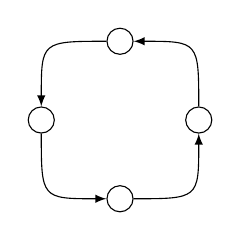
\begin{tikzpicture}
      \tikzstyle{every node}=[circle]
      \node[draw] (n1) at (1,0) {};
      \node[draw] (n2) at (2,1) {};
      \node[draw] (n3) at (1,2) {};
      \node[draw] (n4) at (0,1) {};

      \draw[-latex] (n3) .. controls +(-1,0) .. (n4) {};
      \draw[-latex] (n4) .. controls +(0,-1) .. (n1) {};
      \draw[-latex] (n1) .. controls +(1,0) .. (n2) {};
      \draw[-latex] (n2) .. controls +(0,1) .. (n3) {};
    \end{tikzpicture}\end{tabular} & \begin{tabular}[c]{l} \texttt{x:Node --> .\ --> .\ --> .\ --> x;} \end{tabular}\\
  & \\
  \begin{tabular}[c]{c}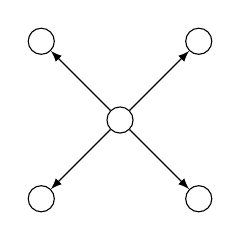
\begin{tikzpicture}
      \tikzstyle{every node}=[circle]
      \node[draw] (n1) at (1,1) {};
      \node[draw] (n2) at (0,0) {};
      \node[draw] (n3) at (0,2) {};
      \node[draw] (n4) at (2,0) {};
      \node[draw] (n5) at (2,2) {};

      \draw[-latex] (n1) -- (n2) {};
      \draw[-latex] (n1) -- (n3) {};
      \draw[-latex] (n1) -- (n4) {};
      \draw[-latex] (n1) -- (n5) {};
    \end{tikzpicture}\end{tabular} & \begin{tabular}[c]{l} \texttt{.\ <-- x:Node --> .;} \\ \texttt{.\ <-- x --> .;} \end{tabular}\\
  & \\
  \begin{tabular}[c]{c}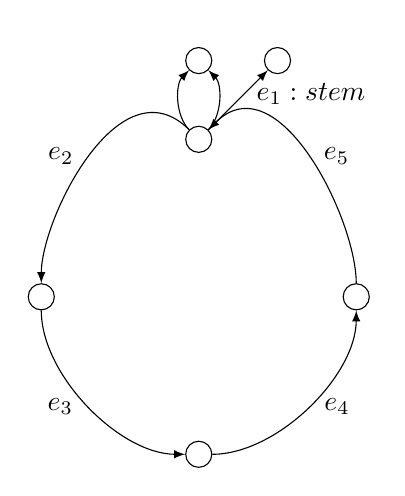
\begin{tikzpicture}
      \tikzstyle{every node}=[circle]
      \node[draw] (n1) at (3,5) {};
      \node[draw] (n2) at (2,4)   {};
      \node[draw] (n3) at (0,2)   {};
      \node[draw] (n4) at (2,0)   {};
      \node[draw] (n5) at (4,2)   {};
      \node[draw] (n6) at (2,5.0)   {};

    	\draw[-latex] (n2) --                                  (n1) node[right,pos=0.6] {$e_1:\text{stem}$};
    	\draw[-latex] (n2) .. controls +(-1,1) and +(0,1) ..   (n3) node[left,midway]  {$e_2$};
      \draw[-latex] (n3) .. controls +(0,-1) and +(-1,0) ..  (n4) node[left,midway]  {$e_3$};
    	\draw[-latex] (n4) .. controls +(1,0)  and +(0,-1) ..  (n5) node[right,midway] {$e_4$};
      \draw[-latex] (n5) .. controls +(0,1)  and +(1,1) ..   (n2) node[right,midway] {$e_5$};
    	\draw[-latex] (n2) .. controls +(-0.3,+0.3) and +(-0.3,-0.3) .. (n6) node[left,midway]   {};
    	\draw[-latex] (n2) .. controls +(+0.3,+0.3) and +(+0.3,-0.3) .. (n6) node[right,midway]  {};
    \end{tikzpicture}\end{tabular} & \begin{tabular}[c]{l} \texttt{.\ <-e1:stem- n1:Node -e2:Edge-> .\ -e3:Edge-> .} \\ \quad\texttt{-e4:Edge-> .\ -e5:Edge-> n1;}\\ \texttt{n1 --> n2:Node;} \\ \texttt{n1 --> n2;} \end{tabular}\\
   & \\
  \begin{tabular}[c]{c}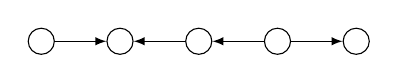
\begin{tikzpicture}
      \tikzstyle{every node}=[circle]
      \node[draw] (n1) at (0,0) {};
      \node[draw] (n2) at (1,0) {};
      \node[draw] (n3) at (2,0) {};
      \node[draw] (n4) at (3,0) {};
      \node[draw] (n5) at (4,0) {};

      \draw[-latex] (n1) -- (n2) {};
      \draw[-latex] (n3) -- (n2) {};
      \draw[-latex] (n4) -- (n3) {};
      \draw[-latex] (n4) -- (n5) {};
    \end{tikzpicture}\end{tabular} & \begin{tabular}[c]{l} \texttt{.\ --> .\ <-- .\ <-- .\ --> .;} \end{tabular} \\
  & \\
  \begin{tabular}[c]{c}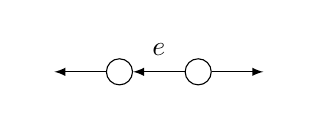
\begin{tikzpicture}
      \tikzstyle{every node}=[circle]
      \node (n1) at (0,0) {};
      \node[draw] (n2) at (1,0) {};
      \node[draw] (n3) at (2,0) {};
      \node (n4) at (3,0) {};

      \draw[-latex] (n2) -- (n1) {};
      \draw[-latex] (n3) -- (n2) node[midway,above] {$e$};
      \draw[-latex] (n3) -- (n4) {};
    \end{tikzpicture}\end{tabular} & \begin{tabular}[c]{l} \texttt{-e:Edge->} \\ \texttt{<-- .\ <-e- .\ -->\ ;} \end{tabular}
\end{tabular}\\
\end{center}
\mbox{ }\\
\mbox{ }\\
\mbox{ }\\
And some illegal graphlets:\\
\mbox{}\\
\mbox{}\\
\begin{tabularx}{\linewidth}{cX}
\texttt{.\ -e:Edge-> .; .\ -e-> .;} & Would affect redirecting of edge \texttt{e}. \\
 & \\
 \texttt{x -e:T-> y; x -e-> x;} & Would affect redirecting of edge \texttt{e}. \\
 & \\
 \texttt{<-- --> ;} & There must be at least a node between the edges.
\end{tabularx}
\end{example}
\end{figure}

\begin{warning}
	Although both, the pattern part and the replace/modify part use graphlets, there are subtle differences between them.
	Most of the differences can be seen in chapter \ref{chapadvanced} where the advanced constructs are explained .
\end{warning}


%%%%%%%%%%%%%%%%%%%%%%%%%%%%%%%%%%%%%%%%%%%%%%%%%%%%%%%%%%%%%%%%%%%%%%%%%%%%%%%%%%%%%%%%%%%%%%%%
\section{Rules and Tests}
\label{ruledecls}
The structure of a \indexed{rule set} file is as follows:
\begin{rail}
  RuleSet: FileHeader ((TestDeclaration | RuleDeclaration | SubpatternDeclaration | RewriteSequenceDefinition | ComputationDefinition)+) ;
  FileHeader: ((ModelUsage)*()) ((RulesInclusion)*()) ((GlobalVarDecl)*());
  ModelUsage: 'using' ((ModelIdent)+',') ';';
  RulesInclusion: '\#include' Filename;
  GlobalVarDecl: '::' IdentDecl ':' NodeType ';' | '-' '::' IdentDecl ':' EdgeType '->' ';' | ('var'|'ref') '::' IdentDecl ':' VarType ';';
\end{rail}\ixkeyw{using}\ixkeyw{include}\ixnterm{RuleSet}\ixnterm{FileHeader}\ixnterm{ModelUsage}\ixnterm{RulesInclusion}\ixnterm{GlobalVarDecl}

A rule set consists of the underlying \indexed{graph model}s and several rewrite rules and tests (subpatterns will be introduced in \ref{sec:subpattern}, rewrite sequence definitions in \ref{sec:sequencedefinition}).
(As a hint regarding the syntax diagrams: please note that the bottom rail in the \emph{RuleSet} diagram departs before the end and joins in after the \emph{FileHeader}, i.e. it denotes a looping back edge (a fast forward edge would have split and join points at the same positions but of the opposite direction)).
Additionally you may \texttt{include} further rule set files (without \texttt{using} directives, we prefer to suffix them with \texttt{.gri} in this case).

Furthermore, you may declare \indexed{graph global variable}s; this is a pure declaration that they will exist with the given type during execution. It renders them accessible in the rules (esp. the attribute condition and attribute evaluation), but you must define and assign them  before rule execution outside of the rules. They are made available to allow for an easy parameterization of entire transformations, defining the environment; other uses are discouraged. See \ref{cha:xgrs} for more on this.
(Use \texttt{ref} for container types and \texttt{var} for the other (non-node or edge) types.)

In case of multiple graph models, \GrG\ uses the union of these models. In this case beware of conflicting declarations.
There is no built-in name conflict resolution mechanism for models like packages or namespaces.
If necessary you must use prefixes as you might do in C.
\footnote{We doubt that graph rewriting kernels will be combined from the work of \emph{many} programmers or used to built large application suites, so the simple model modularization available as of now should be sufficient or even a better fit for the overwhelming majority of tasks.}

\begin{rail}
  TestDeclaration: TestModifier 'test' ActionSignature lbrace Pattern rbrace MatchFilter;
  RuleDeclaration: RuleModifier 'rule' ActionSignature lbrace Pattern Replace rbrace MatchFilter;
\end{rail}\ixkeyw{test}\ixkeyw{rule}\ixkeyw{exact}\ixkeyw{induced}\ixkeyw{dpo}\ixkeyw{dangling}\ixkeyw{identification}\ixnterm{TestDeclaration}\ixnterm{RuleDeclaration}
Declares a single \indexed{rewrite rule} such as \texttt{SomeRule}.
It consists of a pattern part (see Section~\ref{patternpart}) in conjunction with its rewrite/modify part (see Section~\ref{sec:replacemodify}).
A \newterm{test} has no rewrite specification.
It's intended to check whether (and maybe how many times) a pattern occurs (see example \ref{ex:rulelang:testrule}).
For an explanation of the available modifiers see Section~\ref{sct:patternmodifier},
for an explanation of the external match filters see Section~\ref{sub:extflt}.


\begin{example}
\label{ex:rulelang:testrule}
We define a test \texttt{SomeCond}
\begin{grgen}
test SomeCond {
  n:SeldomNodeType;
}
\end{grgen}
and execute in \GrShell:
\begin{grshell}
  exec SomeCond & SomeRule
\end{grshell}
SomeRule will only be executed, if a node of type \texttt{SeldomNodeType} exists.
For graph rewrite sequences in \GrShell\ see Section~\ref{grsthings}.
\end{example}

\begin{rail}
  ActionSignature: IdentDecl (() | Parameters) (() | ':' ReturnTypes) ;
\end{rail}\ixnterm{ActionSignature}
The \indexed{signature} sets the name of a rewrite rule to \emph{IdentDecl} and optionally names and types of formal \indexed{parameter}s as well as a list of \indexed{return type}s.
Parameters and return types provide users with the ability to exchange graph elements between rules, similar to parameters of procedural languages.
This way it is possible to specify \emph{where} a rule should be applied.

\begin{rail}
  Parameters: '(' (Parameter * ',') ')' ;
  Parameter: IdentDecl ':' NodeType (InputTypeSpecification)? | '-' IdentDecl ':' EdgeType (InputTypeSpecification)? '->' | ('var' | 'ref') IdentDecl ':' VarType ;
  InputTypeSpecification: '<' (NodeEdgeType | 'null' | NodeEdgeType '+' 'null' | 'null' '+' NodeEdgeType ) '>' ;
\end{rail}\ixnterm{Parameter}\ixnterm{InputTypeSpecification}\ixkeyw{null}\ixkeyw{var}\ixkeyw{ref}

Within a rule, graph element parameters are treated as graph elements of the pattern - just predefined.
But in contrast to pervious versions it is the task of the user to ensure the elements handed in satisfy the interface, i.e. parameters must not be null and must be of the type specified or a subtype of the type specified.
If you need more flexibility and want to call the rule with parameters not fullfilling the interface you can append an input type specification to the relevant parameters, which consists of the type to accept at the action interface, or null, or both, enclosed in left and right angles.
If the input type specification type is given, but the more specific pattern element type is not satisfied, matching simply fails.
If null is declared in the input type specification and given at runtime, the element is searched in the host graph.
Don't use null parameters unless you need them, because every null parameter doubles the number of matcher routines which get generated.
Non-graph element parameters must be prefixed by the \texttt{var} or \texttt{ref}-keyword;
VarType is one of the attribute types supported by \GrG\ (cf. \ref{sec:builtintypes} and \ref{sec:builtingenerictypes}).
The primitive types require the \texttt{var} prefix and are handed in \indexed{by-value};
the generic types require the \texttt{ref} prefix and are handed in \indexed{by-reference}.
Please note that the effect of assigning to a var/ref parameter in \texttt{eval} (see \ref{sec:replacemodify}) is undefined (concerning the parameters as well as the argument);
they are only available for reading, the by-ref parameters additionally for set/map-addition and removal (cf. \ref{sct:imperative})

\begin{figure}[htbp]
\begin{example}
The \indexed{test} \texttt{t} that checks whether node \texttt{n1} is \indexed{adjacent} to \texttt{n2} (connected by an undirected edge or incoming directed edge or outgoing directed edge)
\begin{grgen}
test t(n1:Node<null>, n2:Node<null>) {
  n1 ?--? n2;
}
\end{grgen}
is equivalent to the tests \texttt{t1}-\texttt{t4} which are chosen dependent on what parameters are defined.
\begin{grgen}
test t1(n1:Node, n2:Node) {
  n1 ?--? n2;
}
test t2(n1:Node) {
  n1 ?--? n2:Node;
}
test t3(n2:Node) {
  n1:Node ?--? n2;
}
test t4 {
  n1:Node ?--? n2:Node;
}
\end{grgen}
So if both parameters are not defined, \texttt{t4} is chosen, which succeeds as soon as there are two distinct nodes in the graph connected by some edge.
\end{example}
\end{figure}

\begin{rail}
  ReturnTypes: '(' ((NodeType | EdgeType | VarType) + ',') ')' ;
\end{rail}\ixnterm{ReturnTypes}
The return types specify edge and node types of graph elements that are returned by the replace/modify part.
If return types are specified, the \texttt{return} statement is mandatory.
Otherwise no \texttt{return} statement must occur. See also Section~\ref{sec:replacemodify}, \texttt{return}.

\begin{figure}[htbp]
\begin{example}\label{ex:rule:someruleext}
We extend \texttt{SomeRule} (Example~\ref{ex:rule:SomeRule}) with a user defined node to match and we want it to return the rewritten graph elements \texttt{n5} and \texttt{e1}.
\begin{grgen}
  rule SomeRuleExt(varnode:Node):(Node, EdgeTypeB) {
    n1:NodeTypeA;
    ...

    replace {
      varnode;
      ...
      return(n5, e1);
      eval {
        ...
\end{grgen}
We do not define \texttt{varnode} within the pattern part because this is already covered by the parameter specification itself.
\end{example}
\end{figure}


%%%%%%%%%%%%%%%%%%%%%%%%%%%%%%%%%%%%%%%%%%%%%%%%%%%%%%%%%%%%%%%%%%%%%%%%%%%%%%%%%%%%%%%%%%%%%%%%
\section{Pattern Part}\indexmain{pattern}
\label{patternpart}
%\begin{rail}
%  Pattern: (() + ('exact' | 'induced')) 'pattern' lbrace (()+PatternStatement) rbrace ;
%\end{rail}\ixkeyw{pattern}\ixkeyw{induced}\ixnterm{Pattern}
\begin{rail}
  Pattern: (()+PatternStatement) (() | ReturnStatement);
\end{rail}\ixnterm{Pattern}
A \indexed{pattern} consists of zero or more pattern statements and, (only) in case of a test, an optional return statement.
All the pattern statements must be fulfilled by a subgraph of the host graph in order to form a match.
An \indexed{empty pattern} always produces exactly one (empty) match.
This is caused by the uniqueness of the total and totally undefined function.
For an explanation of the pattern modifiers \texttt{dpo}, \texttt{identification}, \texttt{dangling}, \texttt{induced}, and \texttt{exact} see Section~\ref{sct:patternmodifier}.

Names defined for graph elements may be used by other pattern statements as well as by replace/modify statements.
Like all identifier definitions, such names may be used before their \indexed{declaration}.
See Section~\ref{rulebb} for a detailed explanation of names and graphlets.
\begin{figure}[htbp]
\begin{warning}
\label{note:indeterminism}
The \indexed{application} of a rule is not deterministic\indexmain{non-determinism}\indexmainsee{determinism}{non-determinism} (remember the example of the introduction in Section~\ref{ov:example}); in particular there may be more than one subgraph that matches the pattern.
Whereas the \GrShell\ selects one of them arbitrarily (without further abilities to control the selection), the underlying \LibGr\indexmain{libGr} provides a mechanism to deal with such ambiguities.

Also notice that graph rewrite \emph{sequences}\indexmain{graph rewrite sequence} introduce a further variant of non-determinism on rule application level:
The \indexed{\texttt{\$<op>}} flag marks the operator \texttt{<op>} as commutative, i.e.\ the execution order of its operands (rules) is non-deterministic.
See Chapter~\ref{cha:xgrs} for further information on graph rewrite sequences.
\end{warning}
\end{figure}

\begin{rail}
  PatternStatement:
    Graphlet ';' |
    HomomorphySpecification ';' |
    ('exact' | 'induced') '(' (Ident+',') ')' |
    'if' lbrace (BooleanExpr ';' +) rbrace |
    'if' '(' BooleanExpr ')' ';'|
    NestedPattern |
    SubpatternEntityDeclaration
    ;
\end{rail}\ixkeyw{induced}\ixkeyw{exact}\ixkeyw{hom}\ixkeyw{if}\ixnterm{PatternStatement}
The semantics of the various pattern statements are given below:
\begin{description}
  \item[Graphlet] \indexmain{graphlet}Graphlets specify connected subgraphs. See Section~\ref{rulebb} for a detailed explanation of graphlets.
  \item[Isomorphic/Homomorphic Matching] See Subsection \ref{rule:homspec} for a discussion of this.
  \item[Attribute Conditions] \indexmain{attribute condition}The Java-like attribute conditions (keyword \texttt{if}) in the pattern part allow for further restriction of the applicability of a rule. The pattern can only match if the \emph{BooleanExpression} (see chapter \ref{cha:typeexpr}) is evaluated to \texttt{true}.
  \item[Pattern Modifiers] Additionally to modifiers that apply to a pattern as a whole, you may also specify pattern modifiers for a specific set of nodes. Accordingly the list of identifiers for a pattern modifier must not contain any edge identifier. See Section~\ref{sct:patternmodifier} for an explanation of the \texttt{exact} and \texttt{induced} modifiers.
  \item[NestedPattern] will be explained in \ref{nac},\ref{pac},\ref{cardinality},\ref{alternative}.
  \item[SubpatternEntityDeclaration] will be explained in \ref{sec:subpattern}.
\end{description}

Keep in mind that using type constraints or the \texttt{typeof} operator might be helpful. See Section~\ref{typeexpressions} for further information.

\begin{rail}
  ReturnStatement: 'return' '(' ((Ident|Expression)+',') ')' ';' ;
\end{rail}\ixkeyw{return}\ixnterm{ReturnStatement}
\indexmain{return value}Returned graph elements (given by their name) and value entities (given by an expression computing them) must appear in the same order as defined by the return types in the signature (see Section~\ref{ruledecls}, \texttt{ActionSignature}).
Their types must be compatible to the return types specified.

\begin{note}
If you are using a graph at the API level without shell-provided names accessible by the \texttt{nameof}-operator, you may want to number the graph elements for dumping like this:
\begin{grgen}
rule numberNode(var id:int) : (int)
{
  n:NodeWithIntId;
  if { n.id == 0; }

  modify {
    eval {
      n.id = id;
    }
    return (id + 1);
  }
}
\end{grgen}
\end{note}


\subsection{Isomorphic and Homomorphic Matching}\label{rule:homspec}\indexmain{isomorphic matching}\indexmain{homomorphic matching}

\begin{rail}
  HomomorphySpecification:
    'hom' '(' (Ident + ',') ')' ';' |
    'independent' '(' Ident (TypeConstraint)? ')' ';'
    ;
\end{rail}\ixkeyw{hom}\ixkeyw{independent}\ixnterm{HomomorphySpecification}

The matching of pattern elements to host graph elements in GrGen.NET is isomorphic (injective) by default, 
i.e. two pattern elements can \emph{not} be bound to the same host graph element.
The \texttt{hom} operator specifies the nodes or edges that may be matched homomorphically.
In contrast to the default isomorphic matching, the specified graph elements \emph{may} be mapped to the same graph element in the host graph. Note that the graph elements must have a common subtype.
Several homomorphically matched graph elements will be mapped to a graph element of a common subtype.
In Example~\ref{ex:rule:SomeRule} nodes \texttt{n1} and \texttt{n2} may be the same node. This is possible because they are of the same type (\texttt{NodeTypeA}).
Inside a NAC/PAC the \texttt{hom} operator may only operate on graph elements that are either defined or used in the NAC/PAC (cf. \ref{nac}/\ref{pac}).
Nested \texttt{negative}/\texttt{independent} blocks inherit the \texttt{hom} declarations of their nesting pattern.
In contrast to previous versions of GrGen \texttt{hom} delarations are non-transitive, i.e \texttt{hom(a,b)} and \texttt{hom(b,c)} don't cause \texttt{hom(a,c)} unless specified.

The \texttt{independent} operator specifies the node or edge given within the parentheses to be homomorphic to all the other pattern elements.
With the constraint clause following, exceptions can be given defining the pattern elements it must be distinct to.
Thus we got a specification mode requesting homomorphic matching with additional isomorphy exceptions in contrast to the default mode,
requesting isomorphic matching with additional homomorphy exception.
It is recommended to \emph{not} use the \texttt{independent} operator, it it potentially dangerous allowing to carry out conflicting rewrites, with an element \texttt{a} to be deleted, element \texttt{b} to be kept, and element \texttt{c} to be retyped, all mapping to the same graph element (you will experience funny effects and/or crashes in this case; the \texttt{hom} operator offers some static checks against this).
The operator is available as a last resort for some situations in matching complex structures with iterated and subpatterns, 
in which it is unfeasible or not possible to explicitely give elements the pattern element may be homomorphic to,
because they were matched in a pattern at an arbitrary distance in the derivation path which only dynamically called the pattern of interest,
i.e. they can't be referenced by name, cf. \ref{locking}.


%%%%%%%%%%%%%%%%%%%%%%%%%%%%%%%%%%%%%%%%%%%%%%%%%%%%%%%%%%%%%%%%%%%%%%%%%%%%%%%%%%%%%%%%%%%%%%%%
\section{Replace/Modify Part}\indexmain{replacement graph}
\label{sec:replacemodify}
Besides specifying the pattern, a main task of a rule is to specify the transformation of a matched subgraph within the \indexed{host graph}.
Such a \indexed{transformation specification} defines the transition from the \indexed{left hand side} (LHS) to the \indexed{right hand side} (RHS), i.e.\ which graph elements of a match will be kept, which of them will be deleted and which graph elements have to be newly created.

%-----------------------------------------------------------------------------------------------
\subsection{Implicit Definition of the Preservation Morphism\indexmain{preservation morphism} $r$}
\label{rule:morphismr}
In theory the transformation specification is done by defining the preservation morphism $r$.
\begin{figure}[htbp]
	\centering
  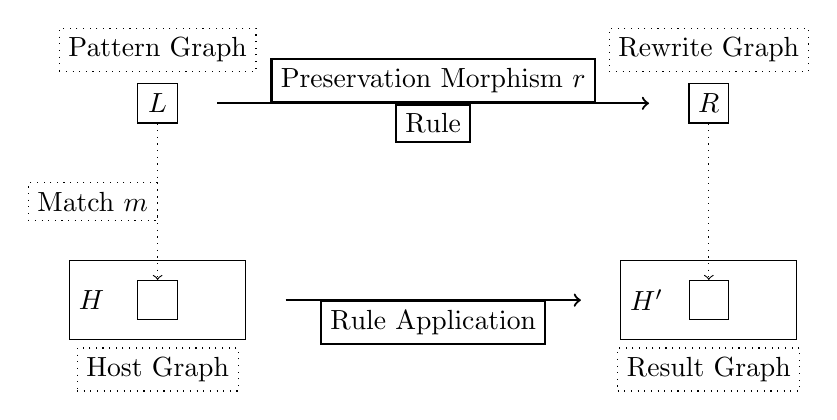
\begin{tikzpicture}
    \begin{scope}[minimum size=0.5cm]
      \tikzstyle{every node}=[draw]
      \node (L)     at (0   ,2.5) {$L$};
      \node (R)     at (7   ,2.5) {$R$};
      \node (mL)    at (0   ,0) {};
      \node (mR)    at (7   ,0) {};
      \node[text width=2cm,text badly ragged,minimum size=1cm] (H)     at (0   ,0) {$H$};
      \node[text width=2cm,text badly ragged,minimum size=1cm] (Hs)    at (7   ,0) {$H'$};
    \end{scope}

    \draw[dotted,->] (L) node[above=0.4cm] {Pattern Graph} -> (mL) node[left,midway]  {Match $m$}   node[below=0.6cm] {Host Graph};
    \draw[dotted,->] (R) node[above=0.4cm] {Rewrite Graph} -> (mR)                              node[below=0.6cm] {Result Graph};

    \pgfsetshortenstart{0.5cm}
    \pgfsetshortenend{0.5cm}
    \draw[thick,->]  (L) -> (R)  node[above,midway] {Preservation Morphism $r$} node[below,midway] {Rule};
    \draw[thick,->]  (H) -> (Hs) node[below,midway] {Rule Application};
  \end{tikzpicture}
  \caption{Process of Graph Transformation}
  \label{rule:figrule}
\end{figure}
In \GrG\, the preservation morphism $r$ is defined implicitly by using \indexed{name}s both in pattern \indexed{graphlet}s and replace graphlets.
Remember that to each of the graph elements a name is bound to, either user defined or internally defined. If such a name is used in a replace graphlet, the denoted graph element will be kept.
Otherwise the graph element will be deleted.
By defining a name in a replace graphlet a corresponding graph element will be newly created.
So in a replace pattern \indexed{anonymous} graph elements will always be created.
Using a name multiple times has the same effect as a single using occurrence.
In case of a conflict between \indexed{deletion} and \indexed{preservation}, deletion is prioritized.
If an incident node of an edge gets deleted, the edge will be deleted as well (in compliance to the SPO\indexmain{single-pushout approach} semantics).

\begin{table}[htbp]
\centering
\begin{tabularx}{\linewidth}{lllX}
  \textbf{Pattern (LHS)} & \textbf{Replace (RHS)} & \textbf{$r: L \longrightarrow R$} & \textbf{Meaning} \\ \hline
  \texttt{x:T;} & \texttt{x;}                 & $r:\lhs.x \mapsto \rhs.x$ & Preservation \\
  \texttt{x:T;} & \texttt{}                   & $\lhs.x \notin \deF(r)$    & Deletion \\
  \texttt{} & \texttt{x:T;}                   & $\rhs.x \notin \ran(r)$    & Creation \\
  \texttt{x:T;} & \texttt{x:T;}               & --- & Illegal, redefinition of \texttt{x} \\
  \texttt{-e:T-> ;} & \texttt{-e-> x:Node;}    & --- & Illegal, redirection of  \texttt{e} \\
  \texttt{x:N -e:E-> y:N;} & \texttt{x -e-> ;} & $r:\{\lhs.x\} \mapsto \{\rhs.x\}$ & Deletion of \texttt{y}. Hence del\-etion of \texttt{e}. \\
\end{tabularx}
\caption{Definition of the preservation morphism $r$}
\label{rule:impldefinition}
\end{table}

%-----------------------------------------------------------------------------------------------
\subsection{Specification Modes for Graph Transformation}
For the task of rewriting, \GrG\ provides two different modes: A \emph{replace mode} and a \emph{modify mode}.
\begin{description}
  \item[Replace mode] \indexmain{replace mode}The semantics of this mode is to delete every graph element of the pattern that is not used (occur) in the replace part, keep every graph element that is used, and create every additionally defined graph elements. ``Using'' means that the name of a graph element occurs in a replace graphlet. Attribute calculations are no using occurrences.\\
  In Example~\ref{ex:rule:someruleext} the nodes \texttt{varnode} and \texttt{n3} will be kept. The node \texttt{n1} is replaced by the node \texttt{n5} preserving \texttt{n1}'s edges. The anonymous edge instance between \texttt{n1} and \texttt{n2} only occurs in the pattern and therefore gets deleted.\\
See Section~\ref{rule:morphismr} for a detailed explanation of the transformation semantics.
  \item[Modify mode] The \indexed{modify mode} can be regarded as a replace part in replace mode, where every pattern graph element is added (occurs) before the first replace statement.
In particular all the \indexed{anonymous} graph elements are kept.
Additionally this mode supports the \texttt{delete} operator that deletes every element given as an argument.
Deletion takes place after all other rewrite operations. Multiple deletion of the same graph element is allowed (but pointless) as well as deletion of just created elements (pointless, too).

\begin{note}
In general modify mode should be prefered as it allows to read the rewrite part as a diff of the changes to be made to the pattern part, whereas replace mode requires comparing the LHS and RHS pattern while reading to find out about the changes.
Only if most of the pattern is to be deleted replace mode is advantageous, pinpointing what should stay.
(Furthermore it might be simpler to generate code for, just dumping both patterns.)
\end{note}

\begin{figure}[htbp]
\begin{example}
How might Example~\ref{ex:rule:someruleext} look in modify mode?
We have to denominate the anonymous edge between \texttt{n1} and \texttt{n2} in order to delete it.
The node \texttt{varnode} should be kept and does not need to appear in the modify part.
So we have
\begin{grgen}
rule SomeRuleExtModify(varnode: Node): (Node, EdgeTypeB)  {
  ...
  n1 -e0:Edge-> n2;
  ...
  modify {
    n5:NodeTypeC<n1>;
    n3 -e1:EdgeTypeB-> n5;
    delete(e0);
    eval {
      ...
\end{grgen}
\end{example}
\end{figure}
\end{description}

%-----------------------------------------------------------------------------------------------
\subsection{Syntax}

\begin{rail}
  Replace: ('replace' | 'modify') lbrace (()+ReplaceStatement) (() | ReturnStatement) \\
  (()+ExecStatement) rbrace ;
\end{rail}\ixkeyw{replace}\ixkeyw{modify}\ixnterm{Replace}\label{replclause}
Selects whether the replace mode or the modify mode is used.
Several replace statements describe the transformation from the pattern subgraph to the destination subgraph.
The \emph{ReturnStatement} was already introduced, for tests it can appear in the pattern part.
Regarding rules it can only be given in the rewrite part.
The \emph{ExecStatement} will be introduced in chapter \ref{cha:imperativeandstate}.

\begin{rail}
  ReplaceStatement:
    Graphlet ';' |
    'delete' '(' (Ident + ',') ')' ';' |
    'eval' lbrace (ComputationStatement +) rbrace |
    SubpatternRewriteApplication
    ;
\end{rail}\ixkeyw{delete}\ixkeyw{eval}\ixnterm{ReplaceStatement}\label{replstmt}
The semantics of the various replace statements are given below:
\begin{description}
  \item[Graphlet] \indexmain{graphlet}Analogous to a pattern graphlet; a specification of a connected subgraph. Its graph elements are either kept because they are elements of the pattern or added otherwise. Names defined in the pattern part must not be redefined in the replace graphlet. See Section~\ref{rulebb} for a detailed explanation of graphlets.
  \item[Deletion] \indexmain{deletion}The \texttt{delete} operator is only available in the modify mode. It deletes the specified pattern graph elements. Multiple occurrences of \texttt{delete} statements are allowed. Deletion statements are executed after all other replace statements. Multiple deletion of the same graph element is allowed (but pointless) as well as deletion of just created elements (pointless, too).
  \item[Computation (Attribute Evaluation)] \indexmain{computation}\indexmainsee{attribute evaluation}{computation}\indexmainsee{evaluation}{attribute evaluation}\indexmainsee{re-evaluation}{attribute evaluation}If a rule is applied, then the attributes of matched and inserted graph elements will be recalculated according to the \texttt{eval} statements. Besides attribute evaluations, further computations may be executed and side effects applied, see Chapter~\ref{cha:computations} for more on this.
  \item[SubpatternRewriteApplication] will be explained in \ref{sec:subrule}.
\end{description}

Several evaluation parts are allowed within the replace part.
Multiple evaluation statements will be internally concatenated, preserving their order.
Evaluation takes place before any graph element specified to be deleted by the rule gets deleted and after all the new elements (according to the rule rewrite part) have been created.
You may read (and write, although this is pointless) attributes of graph elements to be deleted.

\begin{example}
\begin{grgen}
...
modify {
  ...
  eval { y.i = 40; }
  eval { y.j = 0;  }
  x:IJNode;
  y:IJNode;
  delete(x);
  eval {
    x.i = 1;
    y.j = x.i;
    x.i = x.i + 1;
    y.i = y.i + x.i;
  }
}
\end{grgen}
This toy example yields $\texttt{y.i} = 42$, $\texttt{y.j} = 1$.
\end{example}


% todo: graphik die eine beispielregel zeigt und mit pfeilen die konstrukte benennt
